%\pagenumbering{arabic}
\section{系统分析与设计}

\subsection{可行性分析}

可行性分析是对工程项目进行系统技术经济论证,经济合理性综合分析的方法。其基本设计研究目的主要在于通过对我国科学高新技术先进创造水平的高度重视以及程度,经济上的成本合理性及不同条件下继续发展技术可能的不利因素等等进行科学分析和综合论证,选择用最小的减少人力、物力、财务等成本耗费,取得最大和优化的科学技术、经济、社会效益的切实解决方案。它被广泛认为可以是完成项目前期数据分析的一个重要技术手段\upcite{钟珞2005软件工程}。

对于本次开发的软件项目来说,进行可行性分析是必不可少的步骤。可行性研究是对软件项目的一种科学方法,在对于本项目前期经过充分的论证分析后,方可制定计划确保项目实施的进度和控制项目的流程。进而对整个项目进行软件工程的管理。确保了项目具有预见性、公平感、可靠度、科学性。

\subsubsection{经济可行性}

经济的实施可行性主要研究是对本重点工程项目的经济实施可行情况及其进行了技术成本和经济效益的综合分析,从应用市场经济的理论角度,确定是否产出大于投入。以及项目的短期和长期效益方面考虑。

(1)成本角度:

硬件方面本项目主要使用Arduino开发板+各类传感器模块,系统运行在一台2核4G的 kvm 虚拟机之上。相较于其他方案实现,如树莓派,单片机等硬件成本低廉。

软件方面采用开源免费的 Linux 操作系统和 Mysql 数据库,不会产生额外的授权费用。

(2)效益方面:

本系统为相关运维巡检工作减少了经费和资源投入,产生大量可观的直接经济效益和间接经济效益。在提高机房温度智能化监控控制的同时,该系统的可靠与稳定可以保证机房温度的合理性。

本系统的应用切实有效的提高了人员及设备的时间,节省大量时间和经济上的成本,又能提高维护人员工作效率,方便运维管理人员清晰明了的管理各个设备。而且程序的直观表现也能让非专业人员简洁明了地看清各个机房节点的温度、湿度烟雾情况,可以更高效的对于环境进行有理的掌控,便于运维管理人员提出针对性解决方案,避免机房火灾无人发现及温度过高或过低损坏机房电子设备等情况的发生。

\subsubsection{技术可行性}

由于本系统采用C/S模式,对于本系统要从客户端和服务端二个方向去考虑。

客户端方面:

针对于现有的各类开源项目分析,采用Arduino开发板作为分布式节点的客户端无疑是最好的选择,基于Arduino的开发已经非常成熟。不需要关心单片机底层复杂的指令交互逻辑,只需要通过编程语言去控制各组件的输入与输出功能即可。并且和其他类型的单片机相比,有以下优秀的特点:

1. 跨平台---Arduino编程环境可完美兼容当下几乎全部操作系统,不会受到操作系统开发环境对于程序开发的制约和影响。

2. 便宜---Arduino开发板价格非常低廉。一块开发板成本只需要30 RMB,再加装本项目各类所需的传感器之后,成本不会超过100 RMB。

3. 软件硬件开源且可扩展---Arduino以Atmel公司的ATMEGA 8位系列单片机及其SAM3X8E和SAMD21 32位单片机为硬件基础。开发板和模块在遵循“知识共享许可协议\footnote{知识共享许可协议(英语:Creative Commons license,或CC授权)是一种公共版权授权条款,其允许分发受版权保护的作品。一个作者可使用创作共用授权授予他人分享、使用,甚至创作衍生作品的权利。创作共用提供给作者灵活性(例如,他们可以选择允许非商业用途使用他们的作品),保护使用或重新分配他人作品的人,所以他们只要遵守由作者指定的条件,不必担心侵犯版权。}”的前提下发布,所以经验丰富的电路设计人员可以做出属于自己的模块,并进行相应的扩展和改进。即使是经验相对缺乏的用户也可以做出基本Uno开发板,便于了解其运行的原理并节约成本。

4. 简单明了的编程环境---Arduno的开发语言是C语言,非常简单易懂,并且有着大量的示例项目可供参考。

服务端方面:

对于服务端的开发,采用Linux操作系统,选用了Python语言作为主导,Flask模块作为应用程序框架,Mysql作为数据存储,共同构成Web监控管理页面,本人选用了Python语言进行开发,本人之前并无使用Pyhon开发Web界面的经历,本次项目对我来说是一个很大的挑战。

此外,本次系统项目的开发和构建全部在Linux操作系统完成。不同于Windows的臃肿。Linux的哲学: Keep It Simple, Stupid.简洁是Linux遵循的原则。由此可以减少无用项的干扰。

\subsubsection{操作可行性}

本系统除了各分布式节点网络需要修改代码,重新烧录上传Arduino开发板外,其他一切操作基本完成可视化操作,步骤简单,功能清晰,兼顾了实用性和可行性,同时便于运维人员进行系统的管理。

\subsubsection{法律可行性}

本程序依照MIT协议进行发布。被授权人有权利使用、复制、修改、合并、出版发行、散布、再授权和/或贩售软体及软体的副本,及授予被供应人同等权利。对应的义务有在软体和软体的所有副本中都必须包含以上版权声明和本许可声明。依照《中华人民共和国著作法》和《计算机软件保护条例》本系统程序的发布符合中华人民共和国的相关法律。

\subsection{系统需求分析}

目前随着互联网的快速发展,高校的信息化建设进程日益深入,其中数字化校园建设成为其核心内容。纵观全国各高校的数字化校园建设,以建设数字化网络环境、数字化管理手段和工作环境;实现数字化校园和管理;创建数字化生活空间;实现校园的信息化和现代化等为最终目标。为推动数字化校园建设进程,创建数字化管理工作,开发出适用于网络机房的温度监测控制系统,提升校园智能化,数字化进程。通过本系统可以实现智能化、自动化、数字化处理网络机房的温度环境,以智慧化校园为目标进行发展建设\upcite{丁革媛2013数字化网络教学平台的研究与实现}。

根据任务书确立目标,确定基于Arduino的分布式温度温度控制系统的设计采用C/S结构模式。C/S模式是一种普遍应用的网络计算模式。C/S模式是两层结构,在这种模式下,网络中的计算机分为两个有机部分:客户机和服务器。在本次设计中:服务器只负责各种数据的接受和处理,客户端负责数据的采集和传输。在本次设计中客户端具有数据的收集,节点的控制等能力,客户端通过网络使用MQTT协议发送、请求和分析从服务器接收数据。这是一种“瘦客户机(Thin Client)”、“胖服务器(Fat Server)”的网络结构模式。

本系统还提供在线网页查看节点各类信息,以及后台自动处理数据发送邮件报警的功能。此外,本系统使用了API接口,方便做数据的整合,良好的接口设计可以降低系统各部分的相互依赖,提高组成单元的内聚性,降低组成单元间的耦合程度,从而提高系统的维护性和扩展性。同时采用了MQTT数据协议进行数据交互,使得低功耗,多并发,在网络环境差的情况下,网络兼容性好等等优点。

本系统也具有良好的可维护性以及可扩展性。Arduino开发板的使用,可以方便在客户端增加扩展,以Flask为框架,在服务端也可非常容易的做出信息的扩展,采用的ORM数据库读写方式也简单易懂,由于项目涉及方面较为庞大,为了保证他人的共同协作开发,以及后期的二次维护和开发,本项目已在gitee开源。

\subsection{系统整体设计}

本设计主要介绍的是基于Arduino的分布式温度控制系统的主要功能模块的设计与分析。本系统程序设计的根本目标以实现功能需求为基础。采用模块化思想,进行控制。

客户端采用通用的面向过程式的C语言,采用模块化设计,对包括网络通信模块,数据接受处理模块,温度探测模块,红外接受发射模块等四个模块进行了详细的功能构建,结构简单,易于编程实现。

服务端采用Python的Flask框架,具有轻量化和高扩展的特点,另外,在SQL交互方面采用SQLAlchemy \footnote{SQLAlchemy的是Python的SQL工具包和对象关系映射器,可以通过程序代码直接操控SQL数据库}通过ORM\footnote{ORM 就是通过实例对象的语法,完成关系型数据库的操作的技术,是"对象-关系映射"。ORM 把数据库映射成对象}完成数据库的读写,更易于更新和维护以及代码重用,实现了功能的自动完成比如数据的预处理,相比于大量的传统的SQL操作语句ORM代码量少,语义性好,更容易使人理解。


\subsubsection{系统硬件设计}

1. Arduino单片机模块

客户端主要采用图 \ref{fig:2-1} 所示的Arduino开发板进行。其硬件规格为表 \ref{tab1} 所示
\begin{figure}[htbp]
	\centering
	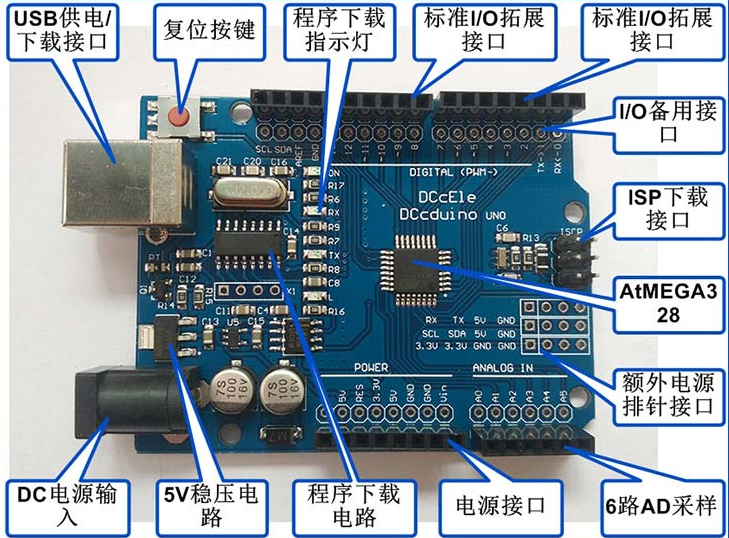
\includegraphics[width=0.85\linewidth]{figure/2-1}
	\caption{Arduino uno 单片机}
	\label{fig:2-1}
\end{figure}
\begin{table}[htbp]
    \centering
	\caption{Arduino uno 硬件规格表}
	\label{tab1}
    \begin{tabular}{|l|l|}
    \hline
		名称 & 规格 \\ \hline
        微控制器 & ATmega328P \\ \hline
        工作电压 & 5V \\ \hline
        输入电压(推荐) & 7-12V \\ \hline
        输入电压(极限) & 6-20V \\ \hline
        数字式的输入和输出引脚 & 14个(其中6个引脚是可以用来作为 pwm 的引脚)\\ \hline
        PWM引脚 & 6个 \\ \hline
        模拟输入引脚 & 6个 \\ \hline
        输入/输出引脚直流电流 & 20 毫安 \\ \hline
        3.3V引脚电流 & 50 毫安 \\ \hline
        Flash Memory(闪存) & 32 KB (ATmega328P) 其中由 0.5 KB用于系统引导(bootloader) \\ \hline
        SRAM(静态存储器) & 2 KB (ATmega328P) \\ \hline
        EEPROM & 1 KB (ATmega328P) \\ \hline
        内置LED引脚 & 13 \\ \hline
        时钟频率 & 16 MHz \\ \hline
    \end{tabular}
\end{table}

2. Arduino扩展模块---Ethernet模块

Ether扩展板如图 \ref{fig:2-2} 主要通过网线负责网络通信和数据传输。W5100模块是一款多功能的单片网络接口芯片,内部集成有10/100M以太网控制器,主要应用于高集成、高稳定、高性能和低成本的嵌入式系统中。在本次设计中通过Ethernet模块,可将传感器数据发送至服务器,完成远程数据信息监控。

\begin{figure}[htbp]
	\centering
	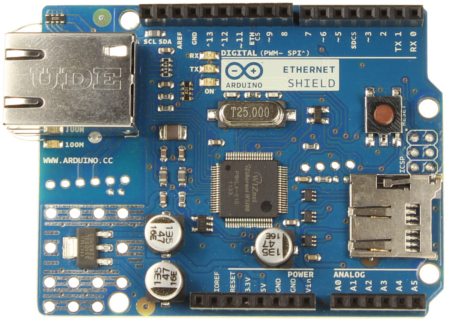
\includegraphics[width=0.85\linewidth]{figure/2-2}
	\caption{Arduino Ethernet 模块}
	\label{fig:2-2}
\end{figure}

3. Arduino传感器模块---DHT11模块,烟雾MQ2模块、红外接收发射模块。

Arduino传感器模块如图 \ref{fig:2-3} 负责监控和控制各个节点的环境信息。

DHT11传感器是一种温湿度复合传感器,包含标定的数字信号输出。采用专用数字化模块化采集技术和温湿度传感器技术,保证了产品极高的可靠性和长期卓越的稳定性。该传感器由电阻式感湿元件和 NTC温度测量元件组成,并与高性能8位单片机相连。这种传感器具有质量优良、响应速度快、抗干扰性强、性价比极高等优点。

MQ-2传感器是基于QM-NG1探针的气体传感器,QM-NG1是一种广谱气体传感器,采用目前国际上工艺最成熟、生产规模最大的\ce{SnO2}材料作为敏感基质制成。其最大特点是对各种易燃气体(如氢、液化气、一氧化碳、烷烃等)和有毒气体(如酒精、乙醚、汽油、烟雾等)高度敏感\upcite{崔阳2014一种基于}。

红外与LED模块是一种与Arduino兼容的红外发射传感器,通过编程发射出38 KHz的调制信号,使其能够适应市场上各种红外遥控器,使红外接收传感器能够接收到发送的信号,从而实现红外无线通信。红外线发射器的核心器件是红外线发射器,广泛应用于红外遥控装置。本模块具有3 PIN接口,通过 Arduino等控制板可以方便地实现红外遥控、通信功能。红外信号遥控器就是利用一个红外线信号发射器向无线控制器发送一连串的数位二进制数字脉冲号来编码控制信号。在无线载波传输的应用过程中,为了有效率地避免其它对所有红外信号的载波干扰,它通常首先工作是在特定的红外载波调制频率上对红外光谱中的信号频率进行载波调制,然后由红外发光二极管的红外发射器探头进行发射。

\begin{figure}[htbp]
	\centering
	\subfigure[DHT11 温湿度传感器模块]{
	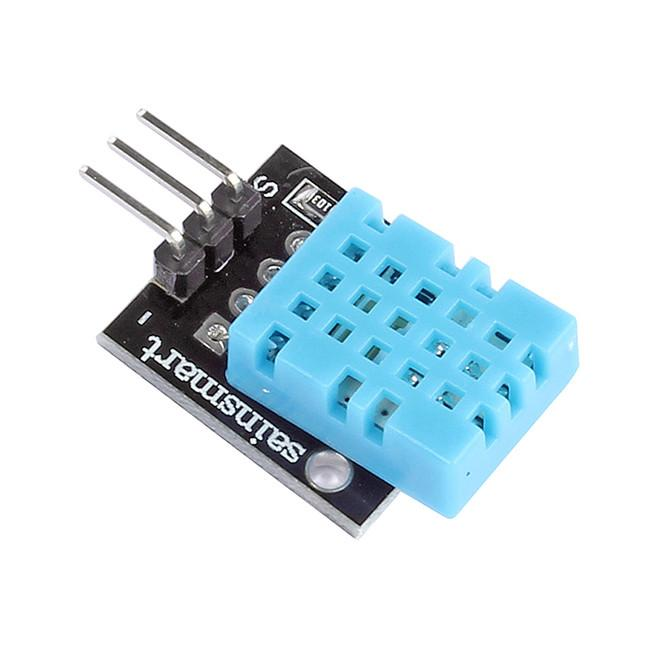
\includegraphics[width=0.3\linewidth]{figure/2-3-1}}
	\subfigure[MQ2 烟雾传感器模块]{
	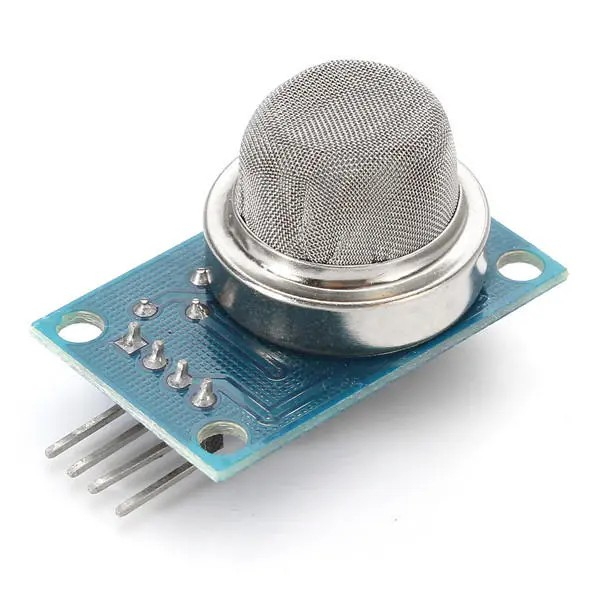
\includegraphics[width=0.3\linewidth]{figure/2-3-2}}
	\subfigure[红外接收发送模块]{
	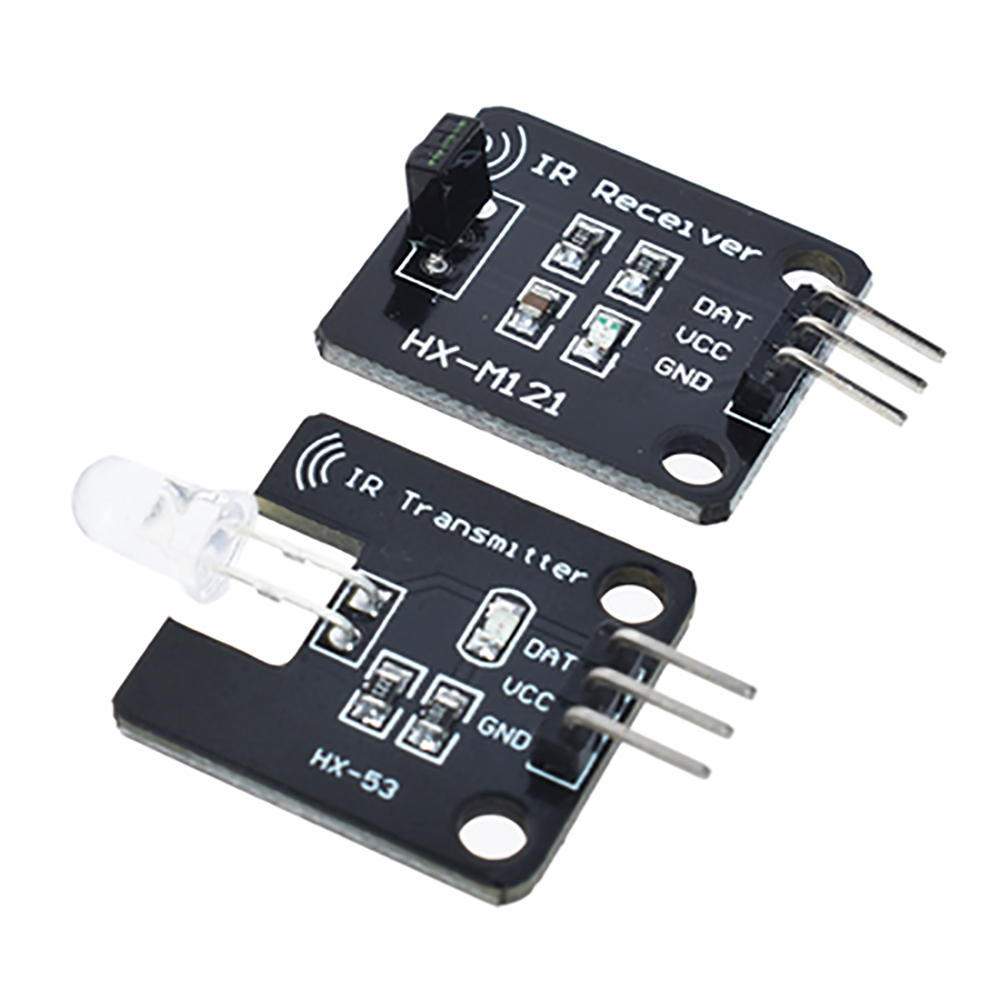
\includegraphics[width=0.3\linewidth]{figure/2-3-3}}
	\caption{传感器模块图}
	\label{fig:2-3}
\end{figure}



\subsubsection{系统架构流程设计}

本系统采用了模块化设计。对实际功能进行模块划分,明确了各模块的功能特征,为以后的开发提供了良好的功能划分。保证了系统输出输入信号的准确一致性,提高了工程设计的系统工作效率,适应性强。按照模块化思想,确立系统的整体架构图如图 \ref{fig:2-4} 所示

\begin{figure}[htbp]
	\centering
	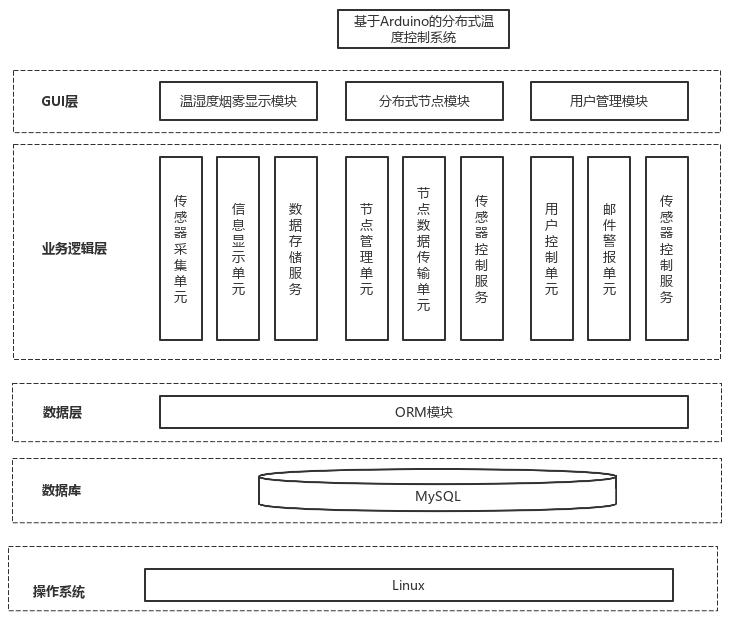
\includegraphics[width=1\linewidth]{figure/2-4}
	\caption{整体架构图}
	\label{fig:2-4}
\end{figure}

数据流图是描述输入数据数据流到输出数据流的变换加工,进而对系统进行整体的功能建模。数据流图用来用于表达系统的逻辑信息流和寻找系统需求,通过简单、以理解的图形符号表达了系统中的据传从输入到存储间所涉及的过程。数据流中通过对数据流、加工、文件、源或宿这些数据元素的表示,反映系统必须完成的逻辑功能,确定功能模型\upcite{王珊珊2008基于}。图 \ref{fig:2-5} 图 \ref{fig:2-6} 所示的客户端服务端交互图是需求分析阶段的成果。

从图中可以看出客户端系统主要由Arduino开发板为中心,通过Arduino开发板附加的各类扩展,完成相应的功能模块。各模块承担信息的收集、发送作用。之后Arduino开发板对数据处理后在以MQTT协议按照与服务端约定的数据格式进行发送。

服务端由MQTT服务器负责接收数据,Flask-MQTT负责数据读取,此时,为了确保数据的及时性,对传入数据立即进行判断,看是否超过设定值,选择是否触发相应警报。之后对对数据附加标注之后存入数据库。之后在由相关的模块从数据库取得各类数据,在前端页面进行可视化展示。

\begin{figure}[htbp]
	\centering
	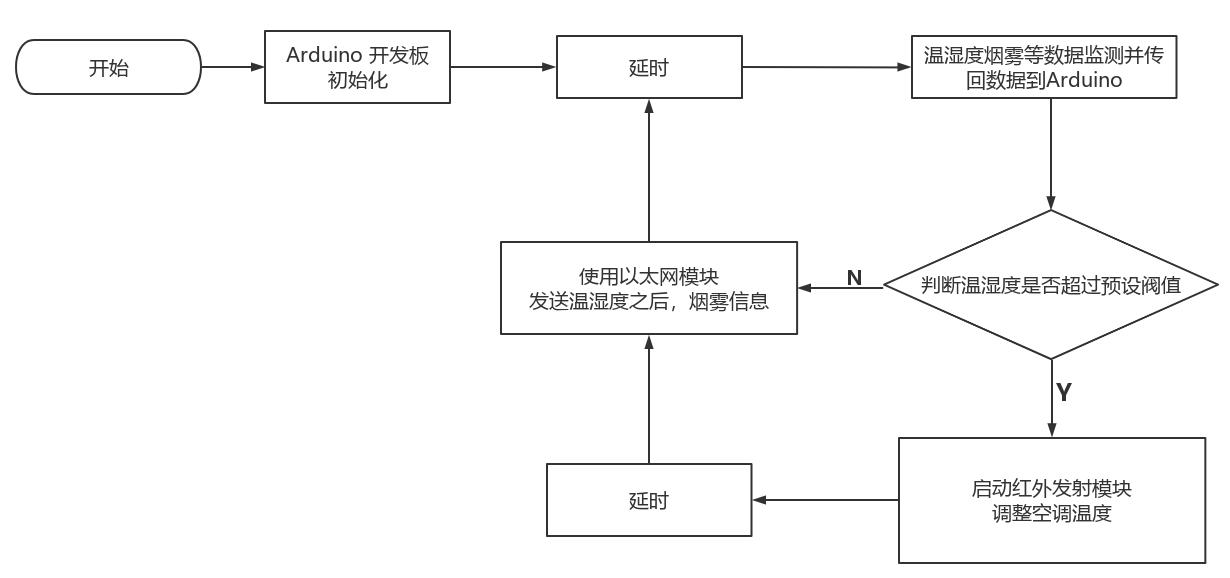
\includegraphics[width=0.85\linewidth]{figure/2-5}
	\caption{Arduino端程序流程图}
	\label{fig:2-5}
\end{figure}

\begin{figure}[htbp]
	\centering
	\subfigure[数据存储流程图]{
	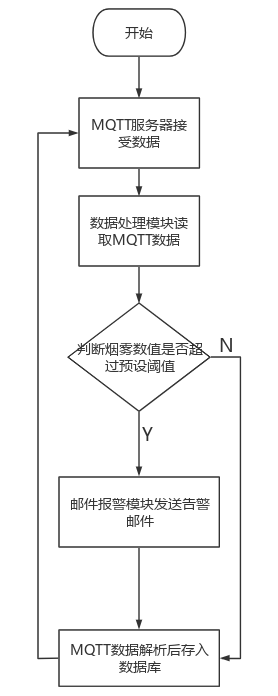
\includegraphics[width=0.4\linewidth]{figure/2-6-1}
	}
	\subfigure[数据展示流程图]{
	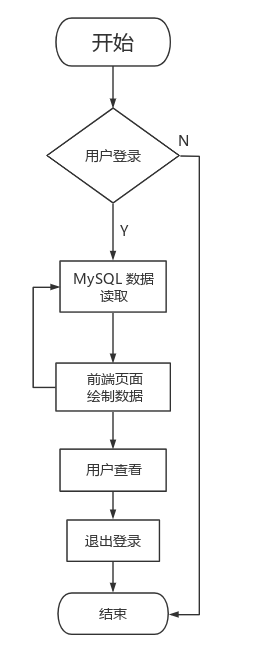
\includegraphics[width=0.4\linewidth]{figure/2-6-2}
	}
	\caption{服务端流程图}
	\label{fig:2-6}
\end{figure}



\subsection{数据库设计}

数据库设计是根据数据库模型组织数据的过程。设计者确定必须存储什么数据以及数据元素是如何相互关联的。有了这些信息,我们就可以开始将数据拟合到数据库模型中。数据库设计涉及分类数据和确定相互关系。这种关于数据的理论表示被称为本体论。本体论是数据库设计背后的理论。

在大多数的情况下,设计一个数据库的工作者都是在业务和设计领域中需要拥有相关专业知识的工作者,而不仅仅需要其他业务和技术领域的相关专业知识。例如,教育经验,从医经验等。因此,数据库的设计必须与在该领域内一定要有专业知识的技术人员进行合作才能确定,以确定必须在系统内存储什么样的数据。这主要是由于一些拥有必须的领域性知识的工作人员往往无法很好地清晰表达自己对于数据库系统需要的信息和技术要求。需要存储的信息可由所需规格来确定。该过程一般被认为是需求分析工作中的一个组成部分。

\begin{figure}[htbp]
	\centering
	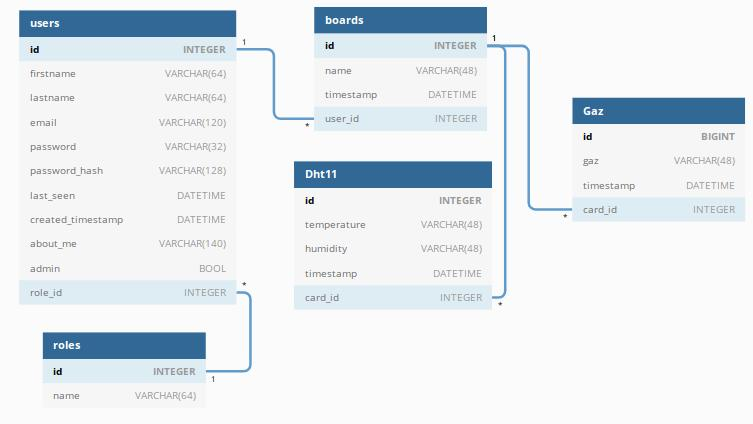
\includegraphics[width=1\linewidth]{figure/2-7}
	\caption{数据库关系图}
	\label{fig:2-7}
\end{figure}

一旦数据库的设计人员确定了他们所需要存放在整个数据库中的所有数据之后,他们必须明确了解到这些数据之间是否具有相互依赖性。例如,在姓名和地址列表中,假设多人可以拥有相同的地址,但一个人不能拥有多个地址的情况下,地址取决于姓名。当提供姓名时,地址可以唯一确定,然而,反过来并不成立。所以在设计数据库时要注意数据库中主键去保证实体完整性。

大多数数据库设计文件采用 
E-R图\footnote{实体 - 关系模型(简称ER模型)描述了描述概念世界。基本的ER模型由实体类型(对感兴趣的事物进行分类)组成,并指定可能存在于这些实体类型的实例之间的关系。}或更直观的矢量图片表示。

本次设计的数据库关系模型如图 \ref{fig:2-7} 所示。本次的数据库设计中,采用了ORM面向对象编程方式进行操作数据库,面向对象编程把所有实体看成对象(object),关系型数据库则是采用实体之间的关系(relation)连接数据。很早就有人提出,关系也可以用对象表达,这样的话,就能使用面向对象编程,来操作关系型数据库。简单说,ORM 就是通过实例对象的语法,完成关系型数据库的操作的技术,是"对象-关系映射"(Object/Relational Mapping)的缩写。其中映射关系为:
\\ 1. 数据库的表(table)对应编程语言中的类(class)
\\ 2. 数据库中的记录(record,行数据)对应编程语言中的对象(object) 
\\ 3. 数据库中的字段(field)对应编程语言中的对象的属性(attribute)

下面以图 \ref{fig:2-7} 中以User表的建立来举例:通过ORM的使用,与传统数据库操作比较就可以发现,ORM 使用对象,封装了数据库操作,因此可以不编写 SQL 语句。开发者只使用面向对象编程,与数据对象直接交互,不用关心底层数据库,屏蔽了数据库之间的差异。

项目代码通常会使用诸如Git\footnote{Git 是一个版本控制系统,用于跟踪计算机文件中的变化并协调多人之间的这些文件的工作。在后文还会详细介绍本项目基于 Git 的团队协作工作流。}、SVN\footnote{SVN使用起来有点像是档案仓库的感觉,支持并行读写文件,支持代码的版本化管理,功能包括取出、导入、更新、分支、改名、还原、合并等。}等版本控制工具管理起来,其好处众所周知,一个是代码多版本管理,另一个是多人协作开发。在项目的持续进展中,数据库的模式(Schema)通常也经常需要更新,比如增加一个表、增加一个列或者创建一个索引等。当新版本升级发布时,在部署阶段,我们需要一个工具能够记录数据库变更版本,类似Git一样能够随时checkout到指定的数据库版本,支持upgrade以及downgrade。我们连接数据库的driver通常称为引擎(engine),这些引擎是抽象接口,其驱动的具体实现可以是mysql、sqlite等关系数据库,实际部署时通过配置的connection协议区分。因此我们的工具应该不依赖于某个具体数据库,而应该是一个通用的工具,屏蔽底层数据库的差别。而支持SQLAlchemy数据库model变更的工具我们称为数据库版本管理工具,或者称为Migrate工具。所有涉及的数据库模式变更脚本都放到称为migrate repository目录中。目前主流的两大主流Migrate工具分别为SQLAlchemy Migrate和Alembic。本次通过使用Alembic引入了可控制数据库版本的特性。

\begin{lstlisting}
op.create_table('users',
sa.Column('id', sa.Integer(), nullable=False),
sa.Column('firstname', sa.String(length=64), nullable=True),
sa.Column('lastname', sa.String(length=64), nullable=True),
sa.Column('email', sa.String(length=120), nullable=True),
sa.Column('password', sa.String(length=32), nullable=True),
sa.Column('password_hash', sa.String(length=128), nullable=True),
sa.Column('last_seen', sa.DateTime(), nullable=True),
sa.Column('created_timestamp', sa.DateTime(), nullable=True),
sa.Column('about_me', sa.String(length=140), nullable=True),
sa.Column('admin', sa.Boolean(), nullable=True),
sa.Column('role_id', sa.Integer(), nullable=True),
sa.ForeignKeyConstraint(['role_id'], ['roles.id'], ),
sa.PrimaryKeyConstraint('id')
)
\end{lstlisting}

